% Options for packages loaded elsewhere
\PassOptionsToPackage{unicode}{hyperref}
\PassOptionsToPackage{hyphens}{url}
\PassOptionsToPackage{dvipsnames,svgnames,x11names}{xcolor}
%
\documentclass[
  letterpaper,
  DIV=11,
  numbers=noendperiod]{scrartcl}

\usepackage{amsmath,amssymb}
\usepackage{lmodern}
\usepackage{iftex}
\ifPDFTeX
  \usepackage[T1]{fontenc}
  \usepackage[utf8]{inputenc}
  \usepackage{textcomp} % provide euro and other symbols
\else % if luatex or xetex
  \usepackage{unicode-math}
  \defaultfontfeatures{Scale=MatchLowercase}
  \defaultfontfeatures[\rmfamily]{Ligatures=TeX,Scale=1}
\fi
% Use upquote if available, for straight quotes in verbatim environments
\IfFileExists{upquote.sty}{\usepackage{upquote}}{}
\IfFileExists{microtype.sty}{% use microtype if available
  \usepackage[]{microtype}
  \UseMicrotypeSet[protrusion]{basicmath} % disable protrusion for tt fonts
}{}
\makeatletter
\@ifundefined{KOMAClassName}{% if non-KOMA class
  \IfFileExists{parskip.sty}{%
    \usepackage{parskip}
  }{% else
    \setlength{\parindent}{0pt}
    \setlength{\parskip}{6pt plus 2pt minus 1pt}}
}{% if KOMA class
  \KOMAoptions{parskip=half}}
\makeatother
\usepackage{xcolor}
\setlength{\emergencystretch}{3em} % prevent overfull lines
\setcounter{secnumdepth}{-\maxdimen} % remove section numbering
% Make \paragraph and \subparagraph free-standing
\ifx\paragraph\undefined\else
  \let\oldparagraph\paragraph
  \renewcommand{\paragraph}[1]{\oldparagraph{#1}\mbox{}}
\fi
\ifx\subparagraph\undefined\else
  \let\oldsubparagraph\subparagraph
  \renewcommand{\subparagraph}[1]{\oldsubparagraph{#1}\mbox{}}
\fi

\usepackage{color}
\usepackage{fancyvrb}
\newcommand{\VerbBar}{|}
\newcommand{\VERB}{\Verb[commandchars=\\\{\}]}
\DefineVerbatimEnvironment{Highlighting}{Verbatim}{commandchars=\\\{\}}
% Add ',fontsize=\small' for more characters per line
\usepackage{framed}
\definecolor{shadecolor}{RGB}{241,243,245}
\newenvironment{Shaded}{\begin{snugshade}}{\end{snugshade}}
\newcommand{\AlertTok}[1]{\textcolor[rgb]{0.68,0.00,0.00}{#1}}
\newcommand{\AnnotationTok}[1]{\textcolor[rgb]{0.37,0.37,0.37}{#1}}
\newcommand{\AttributeTok}[1]{\textcolor[rgb]{0.40,0.45,0.13}{#1}}
\newcommand{\BaseNTok}[1]{\textcolor[rgb]{0.68,0.00,0.00}{#1}}
\newcommand{\BuiltInTok}[1]{\textcolor[rgb]{0.00,0.23,0.31}{#1}}
\newcommand{\CharTok}[1]{\textcolor[rgb]{0.13,0.47,0.30}{#1}}
\newcommand{\CommentTok}[1]{\textcolor[rgb]{0.37,0.37,0.37}{#1}}
\newcommand{\CommentVarTok}[1]{\textcolor[rgb]{0.37,0.37,0.37}{\textit{#1}}}
\newcommand{\ConstantTok}[1]{\textcolor[rgb]{0.56,0.35,0.01}{#1}}
\newcommand{\ControlFlowTok}[1]{\textcolor[rgb]{0.00,0.23,0.31}{#1}}
\newcommand{\DataTypeTok}[1]{\textcolor[rgb]{0.68,0.00,0.00}{#1}}
\newcommand{\DecValTok}[1]{\textcolor[rgb]{0.68,0.00,0.00}{#1}}
\newcommand{\DocumentationTok}[1]{\textcolor[rgb]{0.37,0.37,0.37}{\textit{#1}}}
\newcommand{\ErrorTok}[1]{\textcolor[rgb]{0.68,0.00,0.00}{#1}}
\newcommand{\ExtensionTok}[1]{\textcolor[rgb]{0.00,0.23,0.31}{#1}}
\newcommand{\FloatTok}[1]{\textcolor[rgb]{0.68,0.00,0.00}{#1}}
\newcommand{\FunctionTok}[1]{\textcolor[rgb]{0.28,0.35,0.67}{#1}}
\newcommand{\ImportTok}[1]{\textcolor[rgb]{0.00,0.46,0.62}{#1}}
\newcommand{\InformationTok}[1]{\textcolor[rgb]{0.37,0.37,0.37}{#1}}
\newcommand{\KeywordTok}[1]{\textcolor[rgb]{0.00,0.23,0.31}{#1}}
\newcommand{\NormalTok}[1]{\textcolor[rgb]{0.00,0.23,0.31}{#1}}
\newcommand{\OperatorTok}[1]{\textcolor[rgb]{0.37,0.37,0.37}{#1}}
\newcommand{\OtherTok}[1]{\textcolor[rgb]{0.00,0.23,0.31}{#1}}
\newcommand{\PreprocessorTok}[1]{\textcolor[rgb]{0.68,0.00,0.00}{#1}}
\newcommand{\RegionMarkerTok}[1]{\textcolor[rgb]{0.00,0.23,0.31}{#1}}
\newcommand{\SpecialCharTok}[1]{\textcolor[rgb]{0.37,0.37,0.37}{#1}}
\newcommand{\SpecialStringTok}[1]{\textcolor[rgb]{0.13,0.47,0.30}{#1}}
\newcommand{\StringTok}[1]{\textcolor[rgb]{0.13,0.47,0.30}{#1}}
\newcommand{\VariableTok}[1]{\textcolor[rgb]{0.07,0.07,0.07}{#1}}
\newcommand{\VerbatimStringTok}[1]{\textcolor[rgb]{0.13,0.47,0.30}{#1}}
\newcommand{\WarningTok}[1]{\textcolor[rgb]{0.37,0.37,0.37}{\textit{#1}}}

\providecommand{\tightlist}{%
  \setlength{\itemsep}{0pt}\setlength{\parskip}{0pt}}\usepackage{longtable,booktabs,array}
\usepackage{calc} % for calculating minipage widths
% Correct order of tables after \paragraph or \subparagraph
\usepackage{etoolbox}
\makeatletter
\patchcmd\longtable{\par}{\if@noskipsec\mbox{}\fi\par}{}{}
\makeatother
% Allow footnotes in longtable head/foot
\IfFileExists{footnotehyper.sty}{\usepackage{footnotehyper}}{\usepackage{footnote}}
\makesavenoteenv{longtable}
\usepackage{graphicx}
\makeatletter
\def\maxwidth{\ifdim\Gin@nat@width>\linewidth\linewidth\else\Gin@nat@width\fi}
\def\maxheight{\ifdim\Gin@nat@height>\textheight\textheight\else\Gin@nat@height\fi}
\makeatother
% Scale images if necessary, so that they will not overflow the page
% margins by default, and it is still possible to overwrite the defaults
% using explicit options in \includegraphics[width, height, ...]{}
\setkeys{Gin}{width=\maxwidth,height=\maxheight,keepaspectratio}
% Set default figure placement to htbp
\makeatletter
\def\fps@figure{htbp}
\makeatother

\KOMAoption{captions}{tableheading}
\makeatletter
\makeatother
\makeatletter
\makeatother
\makeatletter
\@ifpackageloaded{caption}{}{\usepackage{caption}}
\AtBeginDocument{%
\ifdefined\contentsname
  \renewcommand*\contentsname{Table of contents}
\else
  \newcommand\contentsname{Table of contents}
\fi
\ifdefined\listfigurename
  \renewcommand*\listfigurename{List of Figures}
\else
  \newcommand\listfigurename{List of Figures}
\fi
\ifdefined\listtablename
  \renewcommand*\listtablename{List of Tables}
\else
  \newcommand\listtablename{List of Tables}
\fi
\ifdefined\figurename
  \renewcommand*\figurename{Figure}
\else
  \newcommand\figurename{Figure}
\fi
\ifdefined\tablename
  \renewcommand*\tablename{Table}
\else
  \newcommand\tablename{Table}
\fi
}
\@ifpackageloaded{float}{}{\usepackage{float}}
\floatstyle{ruled}
\@ifundefined{c@chapter}{\newfloat{codelisting}{h}{lop}}{\newfloat{codelisting}{h}{lop}[chapter]}
\floatname{codelisting}{Listing}
\newcommand*\listoflistings{\listof{codelisting}{List of Listings}}
\makeatother
\makeatletter
\@ifpackageloaded{caption}{}{\usepackage{caption}}
\@ifpackageloaded{subcaption}{}{\usepackage{subcaption}}
\makeatother
\makeatletter
\@ifpackageloaded{tcolorbox}{}{\usepackage[many]{tcolorbox}}
\makeatother
\makeatletter
\@ifundefined{shadecolor}{\definecolor{shadecolor}{rgb}{.97, .97, .97}}
\makeatother
\makeatletter
\makeatother
\ifLuaTeX
  \usepackage{selnolig}  % disable illegal ligatures
\fi
\IfFileExists{bookmark.sty}{\usepackage{bookmark}}{\usepackage{hyperref}}
\IfFileExists{xurl.sty}{\usepackage{xurl}}{} % add URL line breaks if available
\urlstyle{same} % disable monospaced font for URLs
\hypersetup{
  pdftitle={FIFA 21 Analysis},
  pdfauthor={Nathan Weldon},
  colorlinks=true,
  linkcolor={blue},
  filecolor={Maroon},
  citecolor={Blue},
  urlcolor={Blue},
  pdfcreator={LaTeX via pandoc}}

\title{FIFA 21 Analysis}
\author{Nathan Weldon}
\date{}

\begin{document}
\maketitle
\ifdefined\Shaded\renewenvironment{Shaded}{\begin{tcolorbox}[boxrule=0pt, frame hidden, breakable, borderline west={3pt}{0pt}{shadecolor}, enhanced, sharp corners, interior hidden]}{\end{tcolorbox}}\fi

\hypertarget{introduction}{%
\subsection{Introduction}\label{introduction}}

Here, I will load in packages and narrow down what I want to work with
for this data set:

\begin{Shaded}
\begin{Highlighting}[]
\FunctionTok{library}\NormalTok{(tidyverse)}
\end{Highlighting}
\end{Shaded}

\begin{verbatim}
Warning: package 'tidyverse' was built under R version 4.1.2
\end{verbatim}

\begin{Shaded}
\begin{Highlighting}[]
\FunctionTok{library}\NormalTok{(janitor)}

\NormalTok{fifa21\_raw\_data }\OtherTok{\textless{}{-}} \FunctionTok{read\_csv}\NormalTok{(}\StringTok{"\textasciitilde{}/Desktop/Career/Practice/Github/FIFA 21/fifa21\_raw\_data.csv"}\NormalTok{)}

\NormalTok{data }\OtherTok{\textless{}{-}}\NormalTok{ fifa21\_raw\_data }\SpecialCharTok{\%\textgreater{}\%} 
  \FunctionTok{select}\NormalTok{(}\SpecialCharTok{{-}}\FunctionTok{c}\NormalTok{(photoUrl,playerUrl, }\StringTok{\textasciigrave{}}\AttributeTok{Loan Date End}\StringTok{\textasciigrave{}}\NormalTok{, }\StringTok{\textasciigrave{}}\AttributeTok{Release Clause}\StringTok{\textasciigrave{}}\NormalTok{)) }\SpecialCharTok{\%\textgreater{}\%} 
  \FunctionTok{clean\_names}\NormalTok{()}
\end{Highlighting}
\end{Shaded}

\hypertarget{data-synthesis}{%
\subsection{Data Synthesis}\label{data-synthesis}}

Checkout the \texttt{Team\ \&\ Contract} column and separate by how long
they have their contract period and their club. Then, find which players
have played at a club for more than 10 years:

\begin{Shaded}
\begin{Highlighting}[]
\CommentTok{\#clean}
\NormalTok{teamtime }\OtherTok{\textless{}{-}}\NormalTok{ data }\SpecialCharTok{\%\textgreater{}\%} 
  \FunctionTok{drop\_na}\NormalTok{() }\SpecialCharTok{\%\textgreater{}\%} 
  \FunctionTok{mutate}\NormalTok{(}\StringTok{\textquotesingle{}contract\textquotesingle{}} \OtherTok{=} \FunctionTok{str\_sub}\NormalTok{(team\_contract, }\AttributeTok{start =} \SpecialCharTok{{-}}\DecValTok{13}\NormalTok{)) }\SpecialCharTok{\%\textgreater{}\%} 
  \FunctionTok{mutate}\NormalTok{(}\StringTok{\textquotesingle{}team\textquotesingle{}} \OtherTok{=} \FunctionTok{str\_sub}\NormalTok{(team\_contract, }\AttributeTok{start =} \DecValTok{1}\NormalTok{, }\AttributeTok{end =} \SpecialCharTok{{-}}\DecValTok{15}\NormalTok{)) }\SpecialCharTok{\%\textgreater{}\%} 
  \FunctionTok{select}\NormalTok{(}\SpecialCharTok{{-}}\FunctionTok{c}\NormalTok{(team\_contract))}

\CommentTok{\#players 10+ years}
\NormalTok{a }\OtherTok{\textless{}{-}} \FunctionTok{str\_sub}\NormalTok{(teamtime}\SpecialCharTok{$}\NormalTok{contract, }\AttributeTok{start =} \SpecialCharTok{{-}}\DecValTok{4}\NormalTok{, }\AttributeTok{end =} \SpecialCharTok{{-}}\DecValTok{3}\NormalTok{) }\SpecialCharTok{\%\textgreater{}\%} 
  \FunctionTok{as.numeric}\NormalTok{()}
\end{Highlighting}
\end{Shaded}

\begin{verbatim}
Warning in str_sub(teamtime$contract, start = -4, end = -3) %>% as.numeric():
NAs introduced by coercion
\end{verbatim}

\begin{Shaded}
\begin{Highlighting}[]
\NormalTok{b }\OtherTok{\textless{}{-}} \FunctionTok{str\_sub}\NormalTok{(teamtime}\SpecialCharTok{$}\NormalTok{contract, }\AttributeTok{start =} \DecValTok{3}\NormalTok{, }\AttributeTok{end =} \DecValTok{4}\NormalTok{) }\SpecialCharTok{\%\textgreater{}\%} 
  \FunctionTok{as.numeric}\NormalTok{()}
\end{Highlighting}
\end{Shaded}

\begin{verbatim}
Warning in str_sub(teamtime$contract, start = 3, end = 4) %>% as.numeric(): NAs
introduced by coercion
\end{verbatim}

\begin{Shaded}
\begin{Highlighting}[]
\NormalTok{decades }\OtherTok{\textless{}{-}}\NormalTok{ teamtime }\SpecialCharTok{\%\textgreater{}\%} 
  \FunctionTok{mutate}\NormalTok{(}\StringTok{\textquotesingle{}Years\_at\_club\textquotesingle{}}\OtherTok{=}\NormalTok{ a}\SpecialCharTok{{-}}\NormalTok{b) }\SpecialCharTok{\%\textgreater{}\%} 
  \FunctionTok{filter}\NormalTok{(}\FunctionTok{c}\NormalTok{(a}\SpecialCharTok{{-}}\NormalTok{b) }\SpecialCharTok{\textgreater{}=} \DecValTok{10}\NormalTok{) }\SpecialCharTok{\%\textgreater{}\%} 
  \FunctionTok{select}\NormalTok{(}\FunctionTok{c}\NormalTok{(name, Years\_at\_club))}

\FunctionTok{tibble}\NormalTok{(decades)}
\end{Highlighting}
\end{Shaded}

\begin{verbatim}
# A tibble: 462 x 2
   name            Years_at_club
   <chr>                   <dbl>
 1 L. Messi                   17
 2 Casemiro                   10
 3 M. Neuer                   12
 4 K. Benzema                 13
 5 Sergio Ramos               16
 6 S. Agüero                  10
 7 H. Kane                    14
 8 Sergio Busquets            15
 9 H. Lloris                  10
10 G. Chiellini               16
# ... with 452 more rows
\end{verbatim}

\hypertarget{modeling-data}{%
\subsection{Modeling Data}\label{modeling-data}}

Which positions get paid the most? Create a plot that displays this
data:

\begin{Shaded}
\begin{Highlighting}[]
\NormalTok{costs }\OtherTok{\textless{}{-}}\NormalTok{ data }\SpecialCharTok{\%\textgreater{}\%} 
  \FunctionTok{drop\_na}\NormalTok{() }\SpecialCharTok{\%\textgreater{}\%} 
  \FunctionTok{mutate}\NormalTok{(}\StringTok{\textquotesingle{}wage\_thousands\textquotesingle{}} \OtherTok{=} \FunctionTok{str\_extract}\NormalTok{(wage, }\StringTok{"[0{-}9]+}\SpecialCharTok{\textbackslash{}\textbackslash{}}\StringTok{.*[0{-}9]+"}\NormalTok{)) }\SpecialCharTok{\%\textgreater{}\%} 
  \FunctionTok{select}\NormalTok{(}\DecValTok{74}\NormalTok{,bp)}

\NormalTok{worth }\OtherTok{\textless{}{-}}\NormalTok{ costs }\SpecialCharTok{\%\textgreater{}\%} 
  \FunctionTok{drop\_na}\NormalTok{() }\SpecialCharTok{\%\textgreater{}\%}
  \FunctionTok{group\_by}\NormalTok{(bp) }\SpecialCharTok{\%\textgreater{}\%} 
  \FunctionTok{summarize}\NormalTok{(}\StringTok{\textquotesingle{}n\textquotesingle{}} \OtherTok{=} \FunctionTok{mean}\NormalTok{(}\FunctionTok{as.numeric}\NormalTok{(wage\_thousands))) }\SpecialCharTok{\%\textgreater{}\%} 
  \FunctionTok{tibble}\NormalTok{(}\AttributeTok{value =}\NormalTok{ (n }\SpecialCharTok{*} \FloatTok{1.15}\NormalTok{) }\SpecialCharTok{*} \DecValTok{100}\NormalTok{,}
          \AttributeTok{overall =} \FunctionTok{mean}\NormalTok{(bp))}
\end{Highlighting}
\end{Shaded}

\begin{verbatim}
Warning in mean.default(bp): argument is not numeric or logical: returning NA
\end{verbatim}

\begin{Shaded}
\begin{Highlighting}[]
\NormalTok{worth }\SpecialCharTok{\%\textgreater{}\%} \FunctionTok{ggplot}\NormalTok{(}\FunctionTok{aes}\NormalTok{(}\AttributeTok{x =}\NormalTok{ bp, }\AttributeTok{y =}\NormalTok{ value)) }\SpecialCharTok{+} 
  \FunctionTok{geom\_col}\NormalTok{(}\AttributeTok{fill =} \StringTok{\textquotesingle{}chartreuse3\textquotesingle{}}\NormalTok{) }\SpecialCharTok{+}
  \FunctionTok{labs}\NormalTok{(}\AttributeTok{title =} \StringTok{\textquotesingle{}Position vs wage\textquotesingle{}}\NormalTok{,}
       \AttributeTok{subtitle =}\StringTok{\textquotesingle{}Looking at the average wage (USD) per position\textquotesingle{}}\NormalTok{,}
       \AttributeTok{x =} \StringTok{\textquotesingle{}Position\textquotesingle{}}\NormalTok{,}
       \AttributeTok{y =} \StringTok{\textquotesingle{}Average Wage\textquotesingle{}}\NormalTok{)}
\end{Highlighting}
\end{Shaded}

\begin{figure}[H]

{\centering 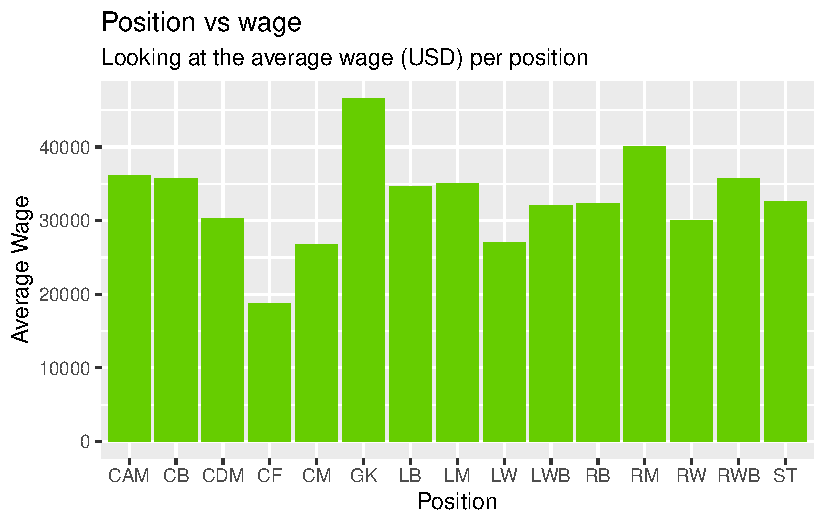
\includegraphics{FIFA21_files/figure-pdf/unnamed-chunk-6-1.pdf}

}

\end{figure}

Let's observe at who is the best technically. Find out who is the best
overall, has the best individual characteristic on a FIFA Card
(pace,shooting, passing, dribbling, defending, physical) and who is the
best overall right / left foot.

\begin{Shaded}
\begin{Highlighting}[]
\CommentTok{\#overall}
\NormalTok{overall }\OtherTok{\textless{}{-}}\NormalTok{ data }\SpecialCharTok{\%\textgreater{}\%} 
  \FunctionTok{drop\_na}\NormalTok{() }\SpecialCharTok{\%\textgreater{}\%} 
  \FunctionTok{filter}\NormalTok{(bp }\SpecialCharTok{!=} \StringTok{\textquotesingle{}GK\textquotesingle{}}\NormalTok{) }\SpecialCharTok{\%\textgreater{}\%} 
  \FunctionTok{filter}\NormalTok{(ova }\SpecialCharTok{==} \FunctionTok{max}\NormalTok{(ova)) }\SpecialCharTok{\%\textgreater{}\%} 
  \FunctionTok{select}\NormalTok{(name, bp, ova) }
\CommentTok{\#pace}
\NormalTok{pace }\OtherTok{\textless{}{-}}\NormalTok{ data }\SpecialCharTok{\%\textgreater{}\%} 
  \FunctionTok{drop\_na}\NormalTok{() }\SpecialCharTok{\%\textgreater{}\%} 
  \FunctionTok{filter}\NormalTok{(bp }\SpecialCharTok{!=} \StringTok{\textquotesingle{}GK\textquotesingle{}}\NormalTok{) }\SpecialCharTok{\%\textgreater{}\%} 
  \FunctionTok{filter}\NormalTok{(pac }\SpecialCharTok{==} \FunctionTok{max}\NormalTok{(pac)) }\SpecialCharTok{\%\textgreater{}\%} 
  \FunctionTok{select}\NormalTok{(name, bp, pac)}
\CommentTok{\#shooting}
\NormalTok{shooting }\OtherTok{\textless{}{-}}\NormalTok{ data }\SpecialCharTok{\%\textgreater{}\%} 
  \FunctionTok{drop\_na}\NormalTok{() }\SpecialCharTok{\%\textgreater{}\%} 
  \FunctionTok{filter}\NormalTok{(bp }\SpecialCharTok{!=} \StringTok{\textquotesingle{}GK\textquotesingle{}}\NormalTok{) }\SpecialCharTok{\%\textgreater{}\%} 
  \FunctionTok{filter}\NormalTok{(sho }\SpecialCharTok{==} \FunctionTok{max}\NormalTok{(sho)) }\SpecialCharTok{\%\textgreater{}\%} 
  \FunctionTok{select}\NormalTok{(name, bp, sho)}
\CommentTok{\#passing}
\NormalTok{passing }\OtherTok{\textless{}{-}}\NormalTok{ data }\SpecialCharTok{\%\textgreater{}\%} 
  \FunctionTok{drop\_na}\NormalTok{() }\SpecialCharTok{\%\textgreater{}\%} 
  \FunctionTok{filter}\NormalTok{(bp }\SpecialCharTok{!=} \StringTok{\textquotesingle{}GK\textquotesingle{}}\NormalTok{) }\SpecialCharTok{\%\textgreater{}\%} 
  \FunctionTok{filter}\NormalTok{(pas }\SpecialCharTok{==} \FunctionTok{max}\NormalTok{(pas)) }\SpecialCharTok{\%\textgreater{}\%} 
  \FunctionTok{select}\NormalTok{(name, bp, pas)}
\CommentTok{\#dribbling}
\NormalTok{dribbling }\OtherTok{\textless{}{-}}\NormalTok{ data }\SpecialCharTok{\%\textgreater{}\%} 
  \FunctionTok{drop\_na}\NormalTok{() }\SpecialCharTok{\%\textgreater{}\%} 
  \FunctionTok{filter}\NormalTok{(bp }\SpecialCharTok{!=} \StringTok{\textquotesingle{}GK\textquotesingle{}}\NormalTok{) }\SpecialCharTok{\%\textgreater{}\%} 
  \FunctionTok{filter}\NormalTok{(dri }\SpecialCharTok{==} \FunctionTok{max}\NormalTok{(dri)) }\SpecialCharTok{\%\textgreater{}\%} 
  \FunctionTok{select}\NormalTok{(name, bp, dri)}
\CommentTok{\#defending }
\NormalTok{defend }\OtherTok{\textless{}{-}}\NormalTok{ data }\SpecialCharTok{\%\textgreater{}\%} 
  \FunctionTok{drop\_na}\NormalTok{() }\SpecialCharTok{\%\textgreater{}\%} 
  \FunctionTok{filter}\NormalTok{(bp }\SpecialCharTok{!=} \StringTok{\textquotesingle{}GK\textquotesingle{}}\NormalTok{) }\SpecialCharTok{\%\textgreater{}\%} 
  \FunctionTok{filter}\NormalTok{(def }\SpecialCharTok{==} \FunctionTok{max}\NormalTok{(def)) }\SpecialCharTok{\%\textgreater{}\%} 
  \FunctionTok{select}\NormalTok{(name, bp, def)}
\CommentTok{\#physical}
\NormalTok{physical }\OtherTok{\textless{}{-}}\NormalTok{ data }\SpecialCharTok{\%\textgreater{}\%} 
  \FunctionTok{drop\_na}\NormalTok{() }\SpecialCharTok{\%\textgreater{}\%} 
  \FunctionTok{filter}\NormalTok{(bp }\SpecialCharTok{!=} \StringTok{\textquotesingle{}GK\textquotesingle{}}\NormalTok{) }\SpecialCharTok{\%\textgreater{}\%} 
  \FunctionTok{filter}\NormalTok{(phy }\SpecialCharTok{==} \FunctionTok{max}\NormalTok{(phy)) }\SpecialCharTok{\%\textgreater{}\%} 
  \FunctionTok{select}\NormalTok{(name, bp, phy)}
\CommentTok{\#right}
\NormalTok{rightf }\OtherTok{\textless{}{-}}\NormalTok{ data }\SpecialCharTok{\%\textgreater{}\%} 
  \FunctionTok{drop\_na}\NormalTok{() }\SpecialCharTok{\%\textgreater{}\%}
  \FunctionTok{filter}\NormalTok{(bp }\SpecialCharTok{!=} \StringTok{\textquotesingle{}GK\textquotesingle{}}\NormalTok{) }\SpecialCharTok{\%\textgreater{}\%} 
  \FunctionTok{filter}\NormalTok{(foot }\SpecialCharTok{==} \StringTok{\textquotesingle{}Right\textquotesingle{}}\NormalTok{) }\SpecialCharTok{\%\textgreater{}\%} 
  \FunctionTok{filter}\NormalTok{(ova }\SpecialCharTok{==} \FunctionTok{max}\NormalTok{(ova)) }\SpecialCharTok{\%\textgreater{}\%} 
  \FunctionTok{select}\NormalTok{(name, foot, ova)}
\CommentTok{\#left}
\NormalTok{leftf }\OtherTok{\textless{}{-}}\NormalTok{ data }\SpecialCharTok{\%\textgreater{}\%} 
  \FunctionTok{drop\_na}\NormalTok{() }\SpecialCharTok{\%\textgreater{}\%}
  \FunctionTok{filter}\NormalTok{(bp }\SpecialCharTok{!=} \StringTok{\textquotesingle{}GK\textquotesingle{}}\NormalTok{) }\SpecialCharTok{\%\textgreater{}\%} 
  \FunctionTok{filter}\NormalTok{(foot }\SpecialCharTok{==} \StringTok{\textquotesingle{}Left\textquotesingle{}}\NormalTok{) }\SpecialCharTok{\%\textgreater{}\%} 
  \FunctionTok{filter}\NormalTok{(ova }\SpecialCharTok{==} \FunctionTok{max}\NormalTok{(ova)) }\SpecialCharTok{\%\textgreater{}\%} 
  \FunctionTok{select}\NormalTok{(name, foot, ova)}

\NormalTok{overall}
\end{Highlighting}
\end{Shaded}

\begin{verbatim}
# A tibble: 1 x 3
  name     bp      ova
  <chr>    <chr> <dbl>
1 L. Messi RW       93
\end{verbatim}

\begin{Shaded}
\begin{Highlighting}[]
\NormalTok{pace}
\end{Highlighting}
\end{Shaded}

\begin{verbatim}
# A tibble: 3 x 3
  name         bp      pac
  <chr>        <chr> <dbl>
1 K. Mbappé    ST       96
2 A. Davies    LB       96
3 Adama Traoré RM       96
\end{verbatim}

\begin{Shaded}
\begin{Highlighting}[]
\NormalTok{shooting}
\end{Highlighting}
\end{Shaded}

\begin{verbatim}
# A tibble: 1 x 3
  name              bp      sho
  <chr>             <chr> <dbl>
1 Cristiano Ronaldo ST       93
\end{verbatim}

\begin{Shaded}
\begin{Highlighting}[]
\NormalTok{passing}
\end{Highlighting}
\end{Shaded}

\begin{verbatim}
# A tibble: 1 x 3
  name         bp      pas
  <chr>        <chr> <dbl>
1 K. De Bruyne CAM      93
\end{verbatim}

\begin{Shaded}
\begin{Highlighting}[]
\NormalTok{dribbling}
\end{Highlighting}
\end{Shaded}

\begin{verbatim}
# A tibble: 1 x 3
  name     bp      dri
  <chr>    <chr> <dbl>
1 L. Messi RW       95
\end{verbatim}

\begin{Shaded}
\begin{Highlighting}[]
\NormalTok{defend}
\end{Highlighting}
\end{Shaded}

\begin{verbatim}
# A tibble: 1 x 3
  name        bp      def
  <chr>       <chr> <dbl>
1 V. van Dijk CB       91
\end{verbatim}

\begin{Shaded}
\begin{Highlighting}[]
\NormalTok{physical}
\end{Highlighting}
\end{Shaded}

\begin{verbatim}
# A tibble: 2 x 3
  name      bp      phy
  <chr>     <chr> <dbl>
1 Casemiro  CDM      91
2 A. Méndez CB       91
\end{verbatim}

\begin{Shaded}
\begin{Highlighting}[]
\NormalTok{rightf}
\end{Highlighting}
\end{Shaded}

\begin{verbatim}
# A tibble: 1 x 3
  name              foot    ova
  <chr>             <chr> <dbl>
1 Cristiano Ronaldo Right    92
\end{verbatim}

\begin{Shaded}
\begin{Highlighting}[]
\NormalTok{leftf}
\end{Highlighting}
\end{Shaded}

\begin{verbatim}
# A tibble: 1 x 3
  name     foot    ova
  <chr>    <chr> <dbl>
1 L. Messi Left     93
\end{verbatim}

\hypertarget{statistical-analysis}{%
\subsection{Statistical Analysis}\label{statistical-analysis}}

Is there a correlation between:

a) age and overall rating?

b) aggression and defending?

c) weight and pace?

d) height and heading?

\begin{Shaded}
\begin{Highlighting}[]
\CommentTok{\#age and overall rating}
\NormalTok{data }\SpecialCharTok{\%\textgreater{}\%} 
  \FunctionTok{ggplot}\NormalTok{(}\AttributeTok{mapping =} \FunctionTok{aes}\NormalTok{(}\AttributeTok{x =}\NormalTok{ age, }\AttributeTok{y =}\NormalTok{ ova, }\AttributeTok{color =}\NormalTok{ foot)) }\SpecialCharTok{+} 
  \FunctionTok{geom\_jitter}\NormalTok{() }
\end{Highlighting}
\end{Shaded}

\begin{figure}[H]

{\centering 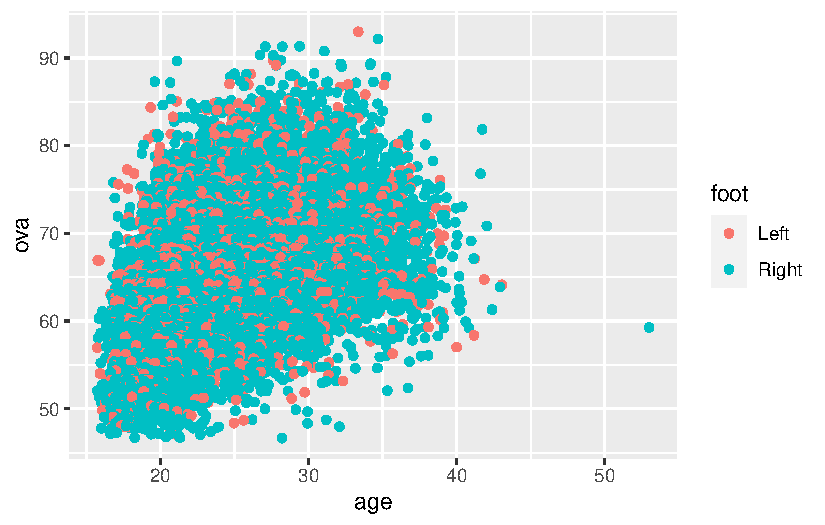
\includegraphics{FIFA21_files/figure-pdf/unnamed-chunk-10-1.pdf}

}

\end{figure}

\begin{Shaded}
\begin{Highlighting}[]
\FunctionTok{cor}\NormalTok{(data}\SpecialCharTok{$}\NormalTok{age, data}\SpecialCharTok{$}\NormalTok{ova)}
\end{Highlighting}
\end{Shaded}

\begin{verbatim}
[1] 0.4662803
\end{verbatim}

\begin{Shaded}
\begin{Highlighting}[]
\NormalTok{m }\OtherTok{\textless{}{-}} \FunctionTok{lm}\NormalTok{(ova }\SpecialCharTok{\textasciitilde{}}\NormalTok{ age, }\AttributeTok{data =}\NormalTok{ data)}
\FunctionTok{summary}\NormalTok{(m)}
\end{Highlighting}
\end{Shaded}

\begin{verbatim}

Call:
lm(formula = ova ~ age, data = data)

Residuals:
     Min       1Q   Median       3Q      Max 
-25.8990  -4.1354  -0.3436   3.7952  27.1748 

Coefficients:
            Estimate Std. Error t value Pr(>|t|)    
(Intercept)  48.3393     0.2435  198.52   <2e-16 ***
age           0.6898     0.0095   72.61   <2e-16 ***
---
Signif. codes:  0 '***' 0.001 '**' 0.01 '*' 0.05 '.' 0.1 ' ' 1

Residual standard error: 6.165 on 18977 degrees of freedom
Multiple R-squared:  0.2174,    Adjusted R-squared:  0.2174 
F-statistic:  5272 on 1 and 18977 DF,  p-value: < 2.2e-16
\end{verbatim}

\emph{Conclusions}:

There seems a moderately strong, positive correlation between age and
the overall rating, in that the older a player is, the higher the rating
will be, on average. From the graph, the points are generally following
this trend confirmed by the correlation being .46. I added in the
dominant foot for the aesthetic and to see if it played a role in the
correlation between the two, and it did not have any noticeable impact.

As for the summary of the model predicting overall rating by using age,
this shows that the R squared is low (.21), meaning the variability of
the data is lacking. In addition, there is a smaller p value than alpha
(\textless2e-16 \textless{} .05), so there is at least some statistical
significant correlation between the two. The coefficient means that for
every year that a player ages, their rating will increase by .69 on
average.

Overall, age is effective in predicting the overall rating of player.

\begin{Shaded}
\begin{Highlighting}[]
\CommentTok{\#aggression and defending}
\NormalTok{data }\SpecialCharTok{\%\textgreater{}\%} 
  \FunctionTok{ggplot}\NormalTok{(}\AttributeTok{mapping =} \FunctionTok{aes}\NormalTok{(}\AttributeTok{x =}\NormalTok{ aggression, }\AttributeTok{y =}\NormalTok{ def)) }\SpecialCharTok{+} 
  \FunctionTok{geom\_jitter}\NormalTok{()}
\end{Highlighting}
\end{Shaded}

\begin{figure}[H]

{\centering 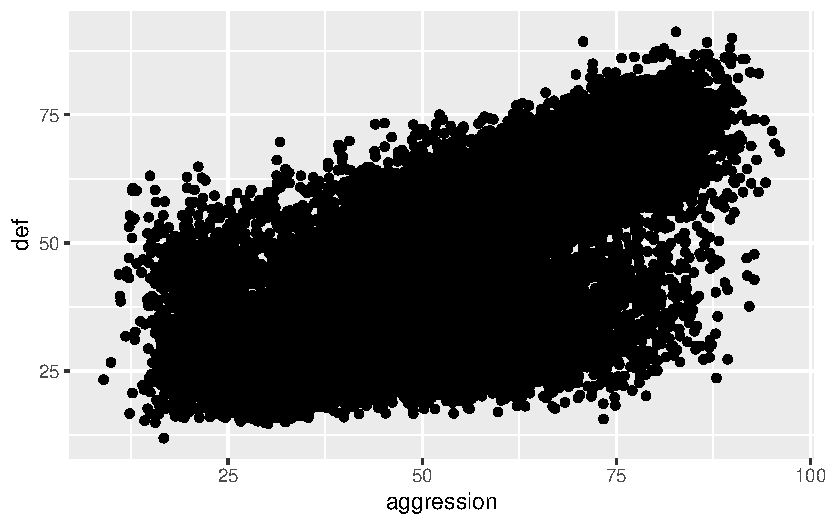
\includegraphics{FIFA21_files/figure-pdf/unnamed-chunk-12-1.pdf}

}

\end{figure}

\begin{Shaded}
\begin{Highlighting}[]
\FunctionTok{cor}\NormalTok{(data}\SpecialCharTok{$}\NormalTok{aggression, data}\SpecialCharTok{$}\NormalTok{def)}
\end{Highlighting}
\end{Shaded}

\begin{verbatim}
[1] 0.6604249
\end{verbatim}

\begin{Shaded}
\begin{Highlighting}[]
\NormalTok{m2 }\OtherTok{\textless{}{-}} \FunctionTok{lm}\NormalTok{(def }\SpecialCharTok{\textasciitilde{}}\NormalTok{ aggression, }\AttributeTok{data =}\NormalTok{ data)}
\FunctionTok{summary}\NormalTok{(m2)}
\end{Highlighting}
\end{Shaded}

\begin{verbatim}

Call:
lm(formula = def ~ aggression, data = data)

Residuals:
    Min      1Q  Median      3Q     Max 
-46.399  -7.889   2.670   8.937  38.851 

Coefficients:
             Estimate Std. Error t value Pr(>|t|)    
(Intercept) 14.645867   0.304193   48.15   <2e-16 ***
aggression   0.633557   0.005229  121.16   <2e-16 ***
---
Signif. codes:  0 '***' 0.001 '**' 0.01 '*' 0.05 '.' 0.1 ' ' 1

Residual standard error: 12.35 on 18977 degrees of freedom
Multiple R-squared:  0.4362,    Adjusted R-squared:  0.4361 
F-statistic: 1.468e+04 on 1 and 18977 DF,  p-value: < 2.2e-16
\end{verbatim}

\emph{Conclusions}:

The data above demonstrates that the more aggressive a player is, the
better defender they will be on average, based on the strong and
positive correlation of .66. In reality this seems to be related because
as a defender, it is imperative that you are aggressive when confronted
with an attacker or a ball that you can win.

The model tells us that there is a statistical significant correlation
when aggression rating predicts the defensive rating since the p value
is significant. The R-squared is moderate, and shows a decent
variability of data at .44. The coefficient is stating that for every
increase in aggression rating, the defensive rating will increase by
.66, for any player on average.

To conclude, there is some influence on the defensive rating from the
aggression rating, in this data set.

\begin{Shaded}
\begin{Highlighting}[]
\CommentTok{\#weight and pace rating}
\NormalTok{paclbs }\OtherTok{\textless{}{-}}\NormalTok{ data }\SpecialCharTok{\%\textgreater{}\%} 
  \FunctionTok{mutate}\NormalTok{(}\StringTok{\textquotesingle{}Weight\textquotesingle{}} \OtherTok{=} \FunctionTok{str\_extract}\NormalTok{(weight, }\StringTok{"[0{-}9]+"}\NormalTok{)) }\SpecialCharTok{\%\textgreater{}\%} 
  \FunctionTok{mutate}\NormalTok{(}\StringTok{\textquotesingle{}lbs\textquotesingle{}} \OtherTok{=} \FunctionTok{as.numeric}\NormalTok{(Weight))}
\NormalTok{paclbs }\SpecialCharTok{\%\textgreater{}\%} 
  \FunctionTok{ggplot}\NormalTok{(}\AttributeTok{mapping =} \FunctionTok{aes}\NormalTok{(}\AttributeTok{x =}\NormalTok{ pac, }\AttributeTok{y =}\NormalTok{ lbs)) }\SpecialCharTok{+} 
  \FunctionTok{geom\_jitter}\NormalTok{()}
\end{Highlighting}
\end{Shaded}

\begin{figure}[H]

{\centering 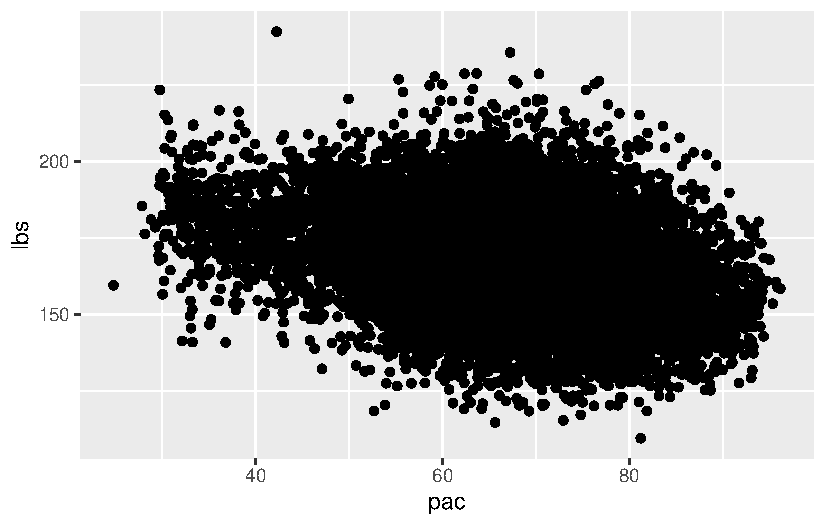
\includegraphics{FIFA21_files/figure-pdf/unnamed-chunk-14-1.pdf}

}

\end{figure}

\begin{Shaded}
\begin{Highlighting}[]
\FunctionTok{cor}\NormalTok{(paclbs}\SpecialCharTok{$}\NormalTok{lbs, paclbs}\SpecialCharTok{$}\NormalTok{pac)}
\end{Highlighting}
\end{Shaded}

\begin{verbatim}
[1] -0.3261879
\end{verbatim}

\begin{Shaded}
\begin{Highlighting}[]
\NormalTok{m3 }\OtherTok{\textless{}{-}} \FunctionTok{lm}\NormalTok{(pac }\SpecialCharTok{\textasciitilde{}}\NormalTok{ lbs, }\AttributeTok{data =}\NormalTok{ paclbs)}
\FunctionTok{summary}\NormalTok{(m3)}
\end{Highlighting}
\end{Shaded}

\begin{verbatim}

Call:
lm(formula = pac ~ lbs, data = paclbs)

Residuals:
    Min      1Q  Median      3Q     Max 
-43.882  -5.988   0.386   6.587  30.034 

Coefficients:
              Estimate Std. Error t value Pr(>|t|)    
(Intercept) 104.409411   0.780883  133.71   <2e-16 ***
lbs          -0.223446   0.004701  -47.53   <2e-16 ***
---
Signif. codes:  0 '***' 0.001 '**' 0.01 '*' 0.05 '.' 0.1 ' ' 1

Residual standard error: 10.09 on 18977 degrees of freedom
Multiple R-squared:  0.1064,    Adjusted R-squared:  0.1064 
F-statistic:  2260 on 1 and 18977 DF,  p-value: < 2.2e-16
\end{verbatim}

\emph{Conclusions}:

This comparison between the weight of a player and how fast the player
is, does not seem to have much magnitude in terms of correlation (-.32).
The negative symbol is interesting, because it means that the less
weight you are, the faster you will be on average, which makes practical
sense as well as the similarity of the graph. I wonder why this would
not be a higher correlation.

The model, where pounds predicts pace, has a variety of useful
statistical information that can be used to create a conclusion. For
instance, the p value being lesser than the alpha value
(\textless2.2e-16 is less than .05), tells us that there is some sort of
correlation between pace rating and weight (in pounds) of a player, on
average. As for the R squared value, it shows how little variability
there is for the data (.106), which does not provide much help when
predicting. The coefficient signifies for every pound that is gained,
the pace rating of a player will decrease by a factor of .22.

Generally, there is some correlation between pace and weight.

\begin{Shaded}
\begin{Highlighting}[]
\CommentTok{\#height and heading}
\NormalTok{inches }\OtherTok{\textless{}{-}}\NormalTok{ data }\SpecialCharTok{\%\textgreater{}\%}
  \FunctionTok{drop\_na}\NormalTok{() }\SpecialCharTok{\%\textgreater{}\%}
  \FunctionTok{mutate}\NormalTok{(}\StringTok{\textquotesingle{}n\textquotesingle{}} \OtherTok{=} \FunctionTok{as.numeric}\NormalTok{(}\FunctionTok{str\_sub}\NormalTok{(height, }\AttributeTok{start=}\DecValTok{1}\NormalTok{, }\AttributeTok{end =} \DecValTok{1}\NormalTok{))) }\SpecialCharTok{\%\textgreater{}\%} 
  \FunctionTok{mutate}\NormalTok{(}\StringTok{\textquotesingle{}n1\textquotesingle{}} \OtherTok{=} \FunctionTok{as.numeric}\NormalTok{(}\FunctionTok{str\_sub}\NormalTok{(height, }\AttributeTok{start =} \DecValTok{3}\NormalTok{, }\AttributeTok{end =} \SpecialCharTok{{-}}\DecValTok{2}\NormalTok{))) }\SpecialCharTok{\%\textgreater{}\%}
  \FunctionTok{mutate}\NormalTok{(}\StringTok{\textquotesingle{}inc\textquotesingle{}} \OtherTok{=}\NormalTok{ (n }\SpecialCharTok{*} \DecValTok{12}\NormalTok{) }\SpecialCharTok{+}\NormalTok{ n1) }\SpecialCharTok{\%\textgreater{}\%}
  \FunctionTok{select}\NormalTok{(heading\_accuracy, n,  n1, inc)}
\NormalTok{inches }\SpecialCharTok{\%\textgreater{}\%} 
  \FunctionTok{ggplot}\NormalTok{(}\AttributeTok{mapping =} \FunctionTok{aes}\NormalTok{(}\AttributeTok{x =}\NormalTok{ heading\_accuracy, }\AttributeTok{y =}\NormalTok{ inc)) }\SpecialCharTok{+}
  \FunctionTok{geom\_jitter}\NormalTok{()}
\end{Highlighting}
\end{Shaded}

\begin{figure}[H]

{\centering 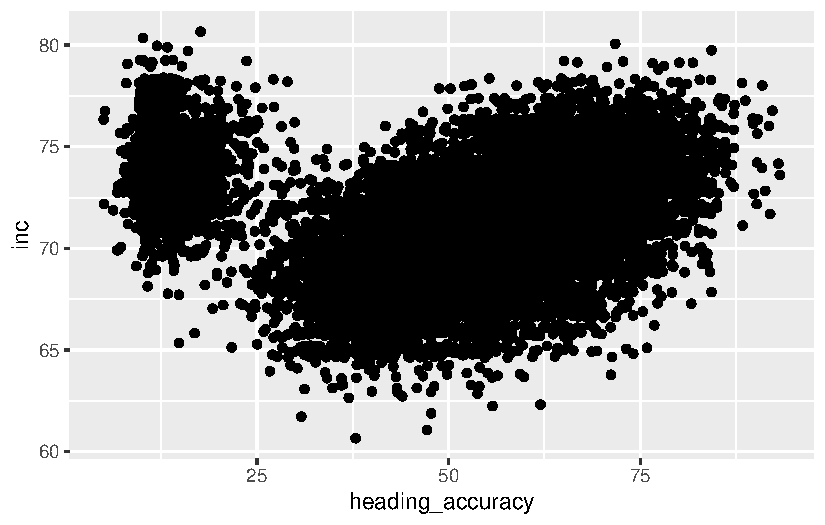
\includegraphics{FIFA21_files/figure-pdf/unnamed-chunk-16-1.pdf}

}

\end{figure}

\begin{Shaded}
\begin{Highlighting}[]
\FunctionTok{cor}\NormalTok{(inches}\SpecialCharTok{$}\NormalTok{heading\_accuracy, inches}\SpecialCharTok{$}\NormalTok{inc)}
\end{Highlighting}
\end{Shaded}

\begin{verbatim}
[1] 0.01102813
\end{verbatim}

\begin{Shaded}
\begin{Highlighting}[]
\NormalTok{m4 }\OtherTok{\textless{}{-}} \FunctionTok{lm}\NormalTok{(heading\_accuracy }\SpecialCharTok{\textasciitilde{}}\NormalTok{ inc, }\AttributeTok{data =}\NormalTok{ inches)}
\FunctionTok{summary}\NormalTok{(m4)}
\end{Highlighting}
\end{Shaded}

\begin{verbatim}

Call:
lm(formula = heading_accuracy ~ inc, data = inches)

Residuals:
    Min      1Q  Median      3Q     Max 
-47.343  -7.775   3.225  12.012  40.870 

Coefficients:
            Estimate Std. Error t value Pr(>|t|)    
(Intercept) 46.87338    3.33845  14.040   <2e-16 ***
inc          0.07104    0.04676   1.519    0.129    
---
Signif. codes:  0 '***' 0.001 '**' 0.01 '*' 0.05 '.' 0.1 ' ' 1

Residual standard error: 17.29 on 18977 degrees of freedom
Multiple R-squared:  0.0001216, Adjusted R-squared:  6.893e-05 
F-statistic: 2.308 on 1 and 18977 DF,  p-value: 0.1287
\end{verbatim}

\emph{Conclusions}:

This data is strange, because it has an incredibly weak correlation
(.01) and the graph explains it, but why there is a grouping of points
almost separate from the bigger trend? Generally, it makes sense that
taller players will have better heading accuracy, yet the grouping on
the left seems to disprove this practical idea of being tall but bad at
heading. The second grouping seems to follow an overall trend that make
logical sense, but is heavily impacted by that first grouping.

This model where the height (in inches) of a player predicts the heading
ability of a player, is not useful for a variety of reasons. For
example, the R squared is tragically below several decimal places below
1, which signifies a very weak variability in the data. The p value
(.12) is greater than alpha (.05), that means that there is no proof
that there is some correlation between the two, statistically. The
coefficient explains that for every inch that a player grows, there will
be an increase in heading accuracy by a rating of .07.

\hypertarget{predicting}{%
\subsection{Predicting}\label{predicting}}

FIFA calculates the overall rating of each player through a variety of
variables. Since there is a lot that goes into each position (ex.
defensive creativity doesn't impact a striker as much as it does a
defender), find a model that predicts the overall rating of only
defenders; choose the variables you think fit a defender best and
simplify the model.



\end{document}
